\documentclass[12pt, a4paper]{article}
\usepackage[margin=1 in]{geometry}
\usepackage{amsmath,amssymb}
\usepackage{enumitem}
\usepackage{hyperref}
\usepackage{graphicx}
\usepackage{appendix}
\usepackage{bm}

\begin{document}
\title{Heading Determination with Tilt Compensation}
\author{Rishav}
\date{June 2021}
\maketitle
\tableofcontents

\newpage
\section{Introduction}
Compass heading determination is a pretty straight forward process. We can compute it by utilizing x-axis and y-axis readings of magnetometer using following equation.

\begin{equation}
    \text{heading} = \tan^{-1}\left(\frac{h_{x}}{h_{y}}\right)
    \label{eqn_heading_basic}
\end{equation}

where, $h_{x}$ and $h_{y}$ are the readings of magnetic field intensity in  x-axis and Y-axis respectively. In order to use this equation we need to make sure that the xy-plane of magnetometer is planar with Earth's surface i.e. we should hold the magnetometer flat with respect to ground  with Z-axis perpendicular to the ground \footnote{Here, \textit{Earth's surface} or \textit{ground} implies flat surface that is parallel to the surface of ideally sphere Earth. If the experiment is performed on slopy land, xy-plane of magnetometer should be perpendicular to the radius vector from centre of the Earth to the magnetometer and not to the sloppy ground.} \cite{honeywell}. \medskip

Eqn.\,(\ref{eqn_heading_basic}) works very well for above mentioned condition, but the magnetometer is not always expected to stay flat in real world applications. For instance, let us suppose a car fitted with magnetometer and we want to track the heading of the car. It is pretty reasonable to assume that we can use Eqn.\,(\ref{eqn_heading_basic}) if we fix the sensor in the car such that xy-plane is parallel to the ground. This assumption wouldnot hold true if the car is moving up or down the hill. In this senario, Eqn.\,(\ref{eqn_heading_basic}) would give incorrect reading of heading. This calls for some correction to Eqn.\,(\ref{eqn_heading_basic}) so that we can use if for real world applications where the sensor tends to tilt. This the goal of this document---to find the tilt compensated heading using magnetometer and accelerometer. We will be using accelerometer to determine the tilt and then use this tilt and magnetometer readings to compute the corrected heading using Eqn.\,(\ref{eqn_heading_basic}). \medskip

The underlying concept and algorithm in this report are those presented in application notes of Freescale Semiconductor \cite{ozyagcilar2015} and \cite{pedley2013}.

\section{Tilt Compensated Heading}

\subsection{Sensor measurements in NED and body frame}

\begin{figure}
    \centering
    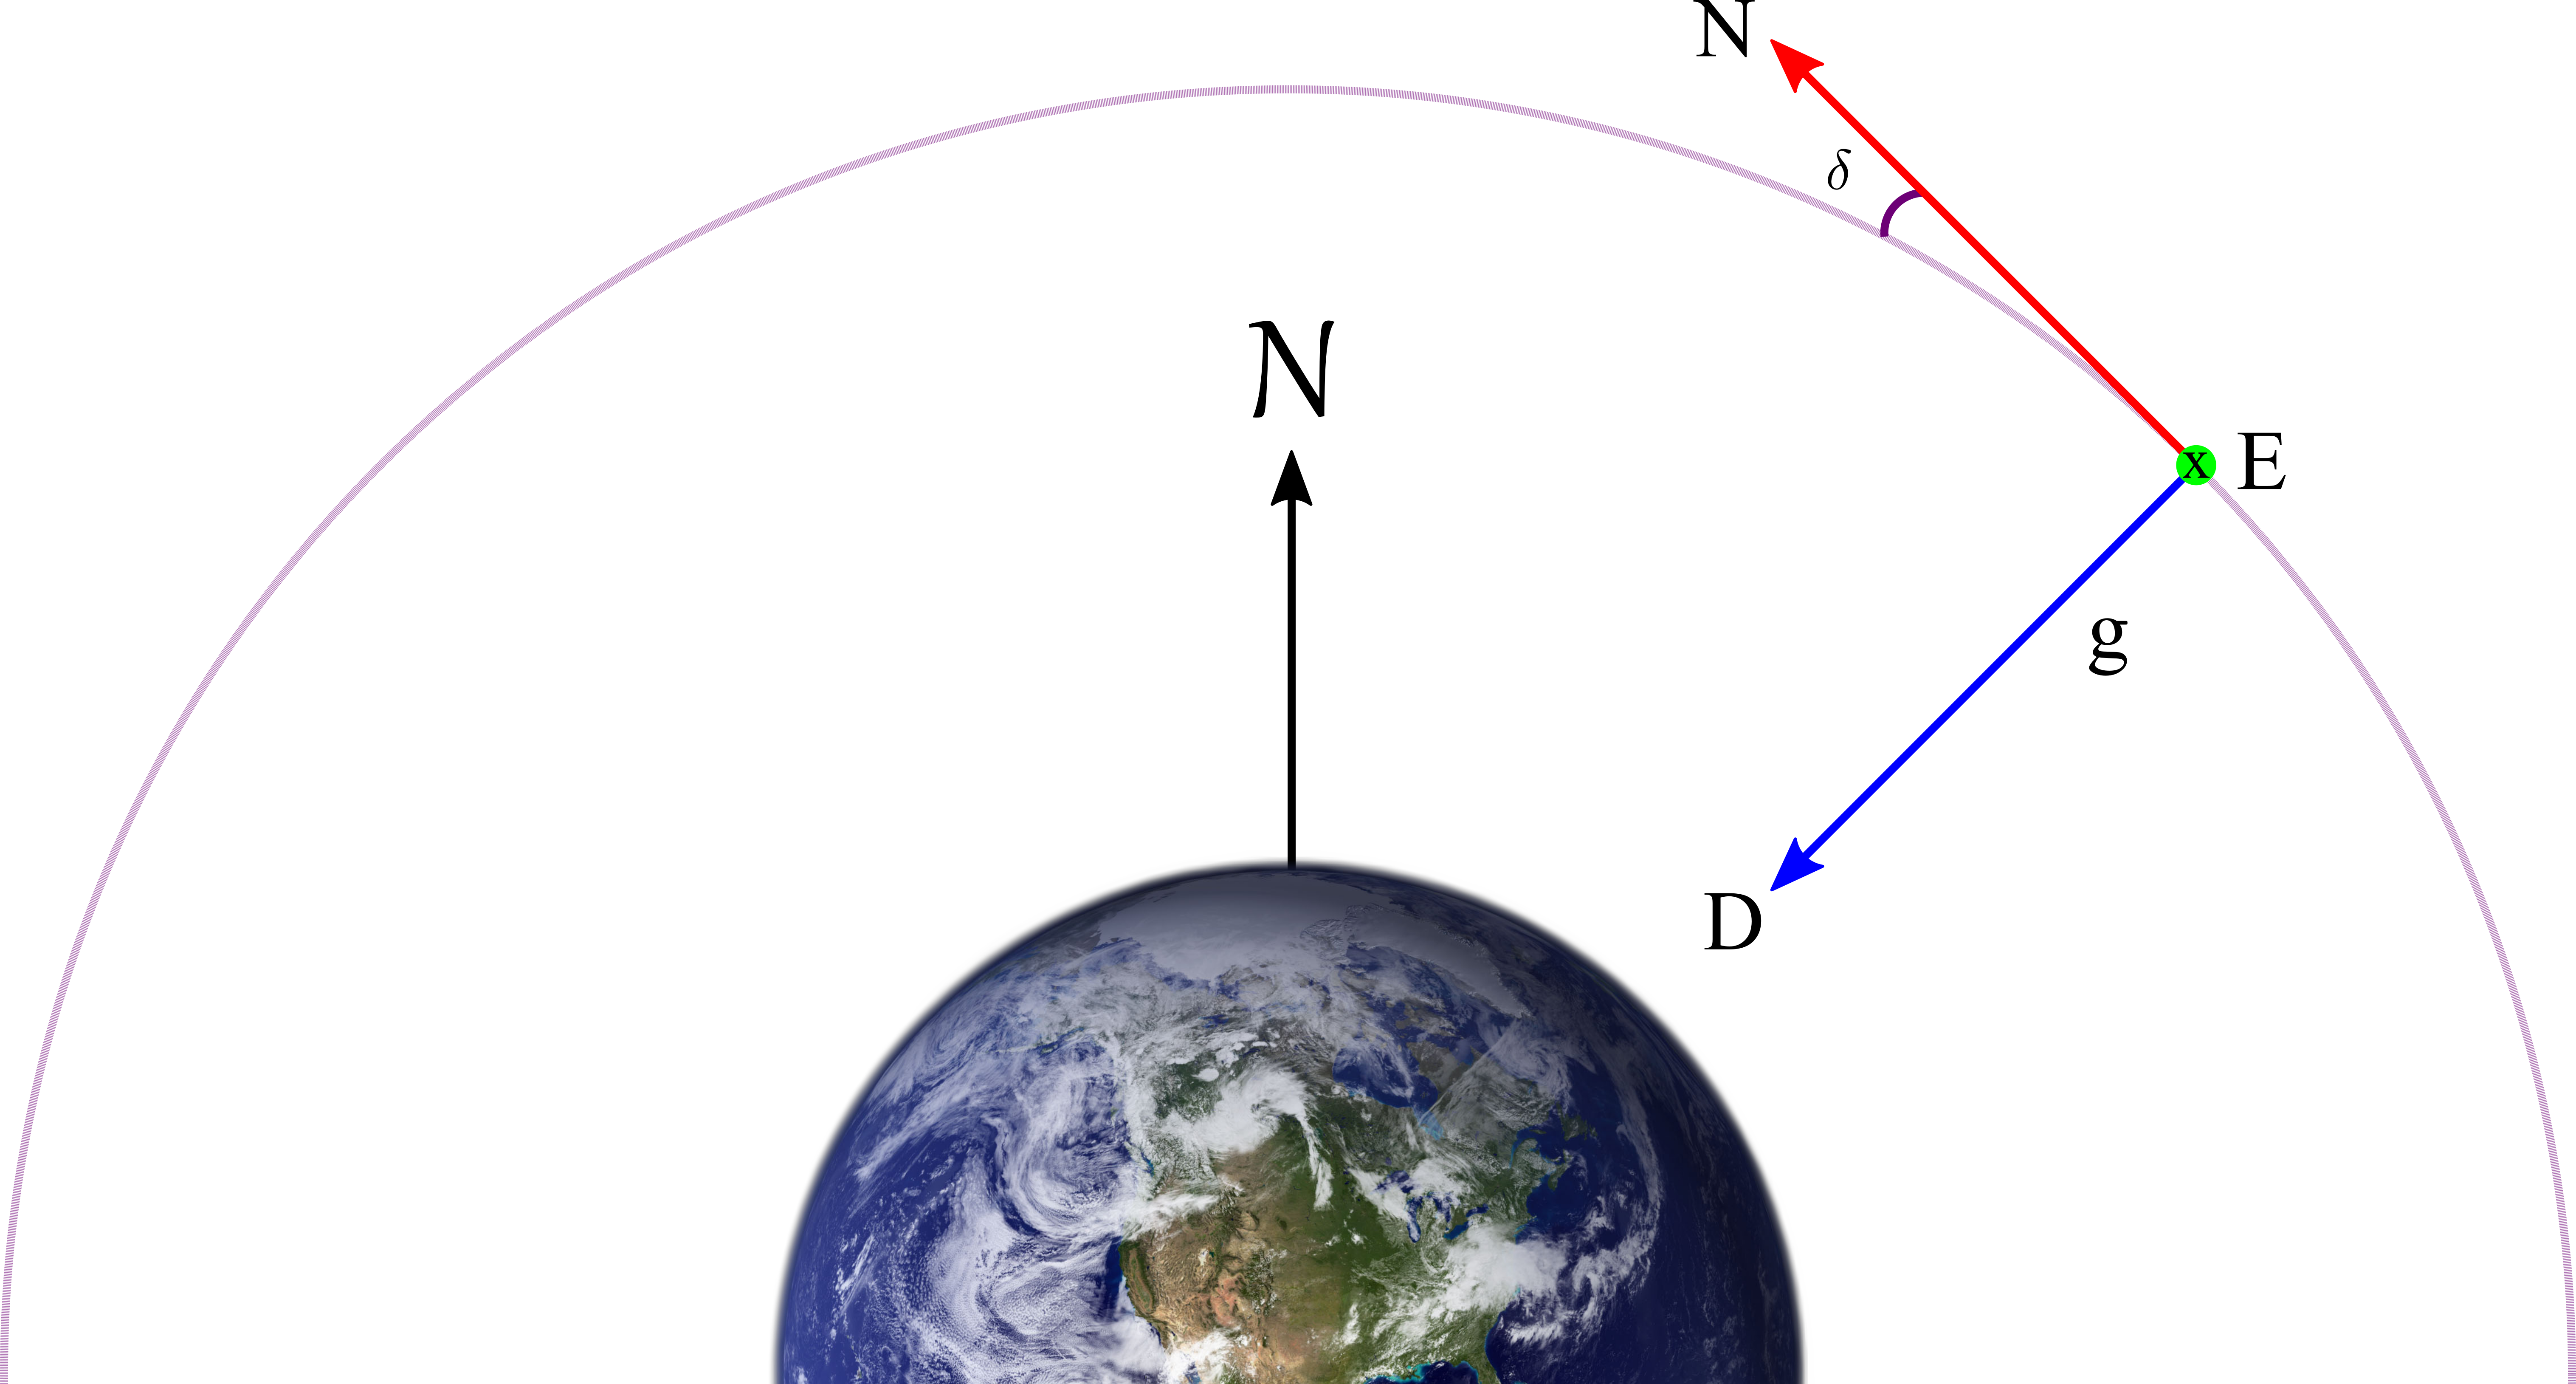
\includegraphics[width=10cm]{figs/fig_ned_frame.png}
    \caption{NED frame with acceleration due to gravity $g$ and magnetic field inclination $\delta$}
\end{figure}

\label{sec_vector_measurements}
Working with the orientation determination using vector measurements \footnote{By \textit{vector measurements}, we mean measurement of physical quantities that exists as field in nature like gravitational field and magnetic fields. The gyroscope readings (angular velocities) are not considered to be vector readings becuase it depends on rotation of body.}  often requires the knowledge of the vectors, that we are measuring, in some known frame of references. Using the vector measurements by sensors in body frame and this knowledge of vectors in some other known frame, the orientation between the two frames of reference is established. \medskip

In this section, we discuss how the magnetometer and accelerometer readings can be intrepreted it the NED frame of reference (See appendix \ref{sec_frames_rotation}).

\subsubsection*{Magnetometer}
We know that magnetic lines of force extend from the North to South. Let $\delta$ be angle of inclination of the geomagnetic field measured downwards from horizontal and varies over
the earth's surface from -90° at the south magnetic pole, through zero near the equator to +90° at the north magnetic pole. In NED frame, the magnetic field vector can be written as $\bm{m}^{N}$.

\begin{equation}
    \bm{m}^{N} = 
    B\begin{bmatrix}\cos\delta \\ 0 \\ \sin\delta\end{bmatrix}
\end{equation}

where, $B$ is the geomagnetic field strength which varies over the
earth's surface. The x and z components of $\bm{m}^{N}$ are the projection of the magnetic field strength in x-axis and y-axis respectively. The y-component (i.e. East component) of the magnetic field in NED is zero because in any given location, there are no components of magnetic field vector in East-West direction.

\subsubsection*{Accelerometer}
The acceleration in NED frame is easier to visualize. Assuming that the sensor itself is not under linear acceleration in any direction, there is only the acceleration due to gravity pointing towards the centre of the Earth. In NED frame, acceleration is present only on z-axis. The acceleration experienced by sensor in NED frame can be written as

\begin{equation}
    \bm{a}^{N} =
    \begin{bmatrix}0 \\ 0 \\ g\end{bmatrix}
\end{equation}

where, $g$ is the acceleration due to gravity in the location where sensor is present. \medskip

We can see that, in this particular problem, if we choose NED as our frame of reference, one component of magnetic field vector and two components of acceleration vector becomes zero. This might not have been the case if we had selected any other arbitrary coordinate frame. This shows that  correct choice of frame of references can help simplify our problem.

\subsection{Problem formulation}
Let us assume $\bm{a}^{B} = [a_{x},\,a_{y},\,a_{z}]^{\intercal}$ and $\bm{m}^{B} = [m_{x},\,m_{y},\,m_{z}]^{\intercal}$  are the three-axes vector measurements by accelerometer and magnetometer respectively in body frame. From the section (\ref{sec_vector_measurements}), we know that the vectors corresponding to $\bm{a}^{B}$ and $\bm{m}^{B}$  in NED frame are $\bm{a}^{N} = [0,\,0,\,g]^{\intercal}$ and $\bm{m}^{N} = [\cos{\delta},\,0,\,\sin{\delta}]^{\intercal}$ respectively. The vectors measured by sensors and the corresponding vectors in NED frame are related by following equations.

\begin{equation}
\begin{split}
\bm{a}^{B} &= \bm{Q}(\psi,\theta,\phi)\,\bm{a}^{N} \\
\bm{m}^{B} &= \bm{Q}(\psi,\theta,\phi)\,\bm{m}^{N} \\
\end{split}
\label{eqn_problem_statement}
\end{equation}

Where, $\bm{Q}(\psi,\theta,\phi)$ is yaw-pitch-roll rotation matrix which is function of Euler angles yaw $\psi$, pitch $\theta$ and roll $\phi$. Detailed study of this matrix is performed in appendix (\ref{sec_ypr}). In Eqn.\,(\ref{eqn_problem_statement}), we know values of $\bm{a}^{B}$ and $\bm{m}^{B}$ from sensor measurements. Similarly, $\bm{a}^{N}(g)$ and $\bm{m}^{N}(\delta)$ can be determined from our location with respect to the Earth. \medskip

In order to find tilt compensated heading, \textit{we are looking for the value of yaw without the effect of roll and pitch}. We will denote tilt compensated yaw by $\tilde{\psi}$. To achieve this task, we will perform three steps: \medskip

\begin{enumerate}[nolistsep]
\item Find $\phi$ and $\theta$ of sensor w.r.t NED using $\bm{a}^{B}$.
\item Rotate \textit{back} $\bm{m}^{B}$ to NED by $\phi$ and $\theta$ using $\bm{Q}^{\intercal}(0,\theta,\phi)$ i.e. $\tilde{\bm{m}} = \bm{Q}^{\intercal}(0,\theta,\phi)\bm{m}^{B}$.
\item Finally, use $\hat{m}_{x}$ and $\tilde{m}_{y}$ to compute $\tilde{\psi}$.
\end{enumerate}

\subsection{Fundamental assumptions}
Before going onto the solution to the problem formulated in above section, we must recognize the fundamental assumptions that allows us to solve the problem by this particular method.

\begin{enumerate}
\item $\bm{a}^{B}$ must function of only $g$ at that place. The accelerometer must not experience any linear accelerations apart from $g$.
\item $\bm{m}^{B}$ should not contain any hard iron or soft iron errors. The magenetometer should be calibrated to get rid those errors.
\item The sensor frame and the body frame must be aligned. Otherwise, there should be an extra step of transforming the sensor readings to the body frame which is not discussed in this report.
\end{enumerate}

\textit{If these assumptions are not valid, then the solution presented in this report does not work}.

\subsection{Roll and pitch determination using accelerometer readings}
From Eqn.\,(\ref{eqn_problem_statement}) we have
\begin{equation}
\bm{a}^{B} = \bm{Q}(\psi,\theta,\phi)\,\bm{a}^{N}
\label{eqn_accel_transformation}
\end{equation}

The resultant rotation produced by $\bm{Q}(\psi,\theta,\phi)$ is composed of there consecutive rotations about Z, Y and X axes respectively.

\begin{equation}
\bm{Q}(\psi,\theta,\phi) = \bm{Q}_{\phi}\,\bm{Q}_{\theta}\,\bm{Q}_{\psi}
\end{equation}

Eq.\,(\ref{eqn_accel_transformation}) can now be written as

\begin{equation}
\bm{a}^{B} = \bm{Q}_{\phi}\,\bm{Q}_{\theta}\,\bm{Q}_{\psi}\,\bm{a}^{N}
\end{equation}

Rotating sensor about Z-axis do not change $\bm{a}^{N} = [0,\,0,\,g]^{\intercal}$ because $\bm{g}$ is along Z-axis. This suggests $\bm{Q}_{\psi}\,\bm{a}^{N} = \bm{a}^{N}$. Using this result, we arrive at

\begin{equation}
\begin{split}
\bm{Q}_{\phi}^{\intercal}\,\bm{Q}_{\theta}^{\intercal}\,\bm{a}^{B} &= \bm{a}^{N} \\
\bm{Q}(0,\theta,\phi)^{\intercal}\,\bm{a}^{B} &= \bm{a}^{N} \\
\end{split}
\label{eqn_tilt_eqn}
\end{equation}

By plugging, $\psi=0$ in the general rotation matrix $\bm{Q}(\phi,\theta,0)$ we get,

\begin{equation}
\bm{Q}(0,\theta,\phi) =
\begin{bmatrix}
\text{c}\theta & 0 & -\text{s}\theta \\
\text{s}\phi\,\text{s}\theta & \text{c}\phi & \text{s}\phi\,\text{c}\theta \\
\text{c}\phi\,\text{s}\theta & -\text{s}\phi & \text{c}\phi\,\text{c}\theta \\
\end{bmatrix} \implies
\bm{Q}(0,\theta,\phi)^{\intercal} =
\begin{bmatrix}
\text{c}\theta & \text{s}\phi\,\text{s}\theta &  \text{c}\phi\,\text{s}\theta \\
0 & \text{c}\phi & -\text{s}\phi \\
-\text{s}\theta& \text{s}\phi\,\text{c}\theta & \text{c}\phi\,\text{c}\theta \\
\end{bmatrix}
\label{eqn_q_transpose}
\end{equation} 

Using Eq.\,(\ref{eqn_tilt_eqn}) and Eq.\,(\ref{eqn_q_transpose}), we get

\begin{equation}
\begin{split}
\begin{bmatrix}
\text{c}\theta & \text{s}\phi\,\text{s}\theta &  \text{c}\phi\,\text{s}\theta \\
0 & \text{c}\phi & -\text{s}\phi \\
-\text{s}\theta & \text{s}\phi\,\text{c}\theta & \text{c}\phi\,\text{c}\theta \\
\end{bmatrix}
\begin{bmatrix}
 a_{x} \\ a_{y} \\ a_{z}
\end{bmatrix}
&=
\begin{bmatrix}
 0 \\ 0 \\ g
\end{bmatrix} \\
\text{or, }
\begin{bmatrix}
a_x\,\text{c}\theta + a_y\,\text{s}\phi\,\text{s}\theta +  a_z\,\text{c}\phi\,\text{s}\theta\\
a_y\,\text{c}\phi -a_z\,\text{s}\phi \\
-a_x\,\text{s}\theta + a_y\,\text{s}\phi\,\text{c}\theta + a_z\,\text{c}\phi\,\text{c}\theta \\
\end{bmatrix} &=
\begin{bmatrix}
 0 \\ 0 \\ g
\end{bmatrix} \\
\end{split}
\label{eqn_tilt_computation}
\end{equation}

Above equation gives two equation which can be solved to get $\phi$ and $\theta$.

\paragraph{Roll determination}
$\phi$ can be determined from Eq.\,({\ref{eqn_tilt_computation}}) using the second equation,

\begin{equation}
\begin{split}
a_{y}\cos{\phi} &- a_{z}\sin{\phi} = 0 \\
\text{or, } \phi &= \tan^{-1}{\left(\cfrac{a_{y}}{a_{z}}\right)} \\
\end{split}
\end{equation}

\paragraph{Pitch determination}
$\theta$ can be determined from Eq.\,({\ref{eqn_tilt_computation}}) using the second equation,

\begin{equation}
\begin{split}
a_{x}\cos{\theta} + &a_{y}\sin{\phi}\sin{\theta} + a_{z}\cos{\phi}\sin{\theta} = 0\\
\theta &= \tan^{-1}{\left(\cfrac{-a_x}{a_y\sin{\phi} + a_z\cos{\phi}}\right)}
\end{split}
\end{equation}

\subsection{Tilt compensation on magnetometer readings}
The tilt ($\phi$ and $\theta$) found using accelerometer is used to produce tilt compensated magnetometer readings and those readings are used to determine $\tilde{\psi}$. To find the tilt compensated magnetometer reading $\tilde{\bm{m}} = [\tilde{m}_{x},\,\tilde{m}_{y},\,\tilde{m}_{z}]^{\intercal}$, we need to rotate back the magnetometer measurement vector $\bm{m}^{B}$ so that the XY-plane of body frame is parallel to the XY-plane of the NED frame. In order to do so, the body frame should be rotated back by $\phi$ and $\theta$. This rotation can me written as,

\begin{equation}
\begin{split}
\tilde{\bm{m}} &= \bm{Q}(0,\theta,\phi)^{\intercal}\,\bm{m}^{B} \\
\begin{bmatrix}
\tilde{m}_{x} \\ \tilde{m}_{y} \\ \tilde{m}_{z}
\end{bmatrix}
&=
\begin{bmatrix}
\text{c}\theta & \text{s}\phi\,\text{s}\theta &  \text{c}\phi\,\text{s}\theta \\
0 & \text{c}\phi & -\text{s}\phi \\
-\text{s}\theta& \text{s}\phi\,\text{c}\theta & \text{c}\phi\,\text{c}\theta \\
\end{bmatrix}
\begin{bmatrix}
 m_{x} \\ m_{y} \\ m_{z}
\end{bmatrix} \\
&=
\begin{bmatrix}
m_x\,\text{c}\theta + m_y\,\text{s}\phi\,\text{s}\theta +  m_z\,\text{c}\phi\,\text{s}\theta\\
m_y\,\text{c}\phi -m_z\,\text{s}\phi \\
-m_x\,\text{s}\theta + m_y\,\text{s}\phi\,\text{c}\theta + m_z\,\text{c}\phi\,\text{c}\theta \\
\end{bmatrix}
\end{split}
\end{equation} 


$\tilde{\bm{m}}$ is used to determine $\tilde{\psi}$.

\begin{equation}
\begin{split}
\tilde{\psi} &= \tan^{-1}{\left(\frac{-\tilde{m_{y}}}{\tilde{m_{x}}}\right)} \\
&= \tan^{-1}{\left(\frac{m_z\,\sin{\phi} - m_y\,\cos{\phi}}{m_x\,\cos{\theta} + m_y\,\sin{\phi}\,\sin{\theta} +  m_z\,\cos{\phi}\,\sin{\theta}}\right)}
\end{split}
\end{equation}

% \section{Some Important Considerations}

% \subsection{Stability of tilt determining equations}
% \subsection{Duplicate solutions and their remedies}

\bibliographystyle{plain}
\bibliography{references}

\appendix
\addcontentsline{toc}{section}{APPENDICES}

\section{Coordinate Frames and Rotations}
\label{sec_frames_rotation}

\subsection{Body frame}

\begin{figure}[h] 
    \centering
    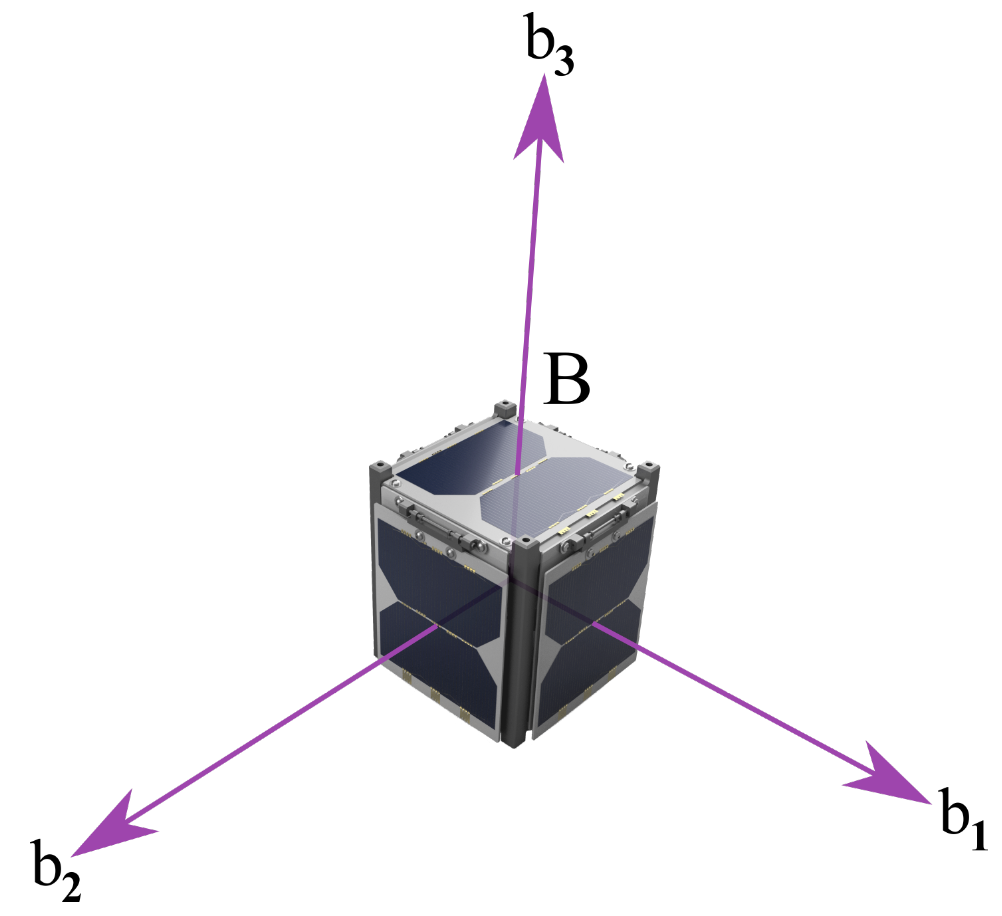
\includegraphics[width=8cm]{figs/fig_body.png}
    \caption{CubeSat body frame (B).}
    \label{fig_body}
\end{figure}

Body frame represents the cartesian coordinate system fixed to the body of the satellite. This means that the body frame revolves around the orbit and rotates with satellite. When we mention the orientaion of satellite, we are actually talking about the orientation of body frame as observed in some inertial frame. \medskip

The simplification of the dynamical equation of the spacecraft requires the body frame to be aligned with the principal axes. This is because the inertia matrix is diagonal in the principal axes, hence a lot of computation is saved. In Fig.\,(\ref{fig_body}), the body frame has its origin in centre of the CubeSat and its axes are perpendicular to the sides of the CubeSat. It is because the mass distribution of the CubeSat is assumed to be such that its inertia matrix is diagonal. Like on all other coordinate systems, the coordinate axes of the body frame B are defined with mutually orthogonal unit vectors $\hat{\bm{b}}_{1}$, $\hat{\bm{b}}_{2}$ and $\hat{\bm{b}}_{3}$ in the direction of  $b_{1}$, $b_{2}$ and $b_{3}$ axes respectively.\medskip

\subsection{NED frame}

\begin{figure}[h] 
    \centering
    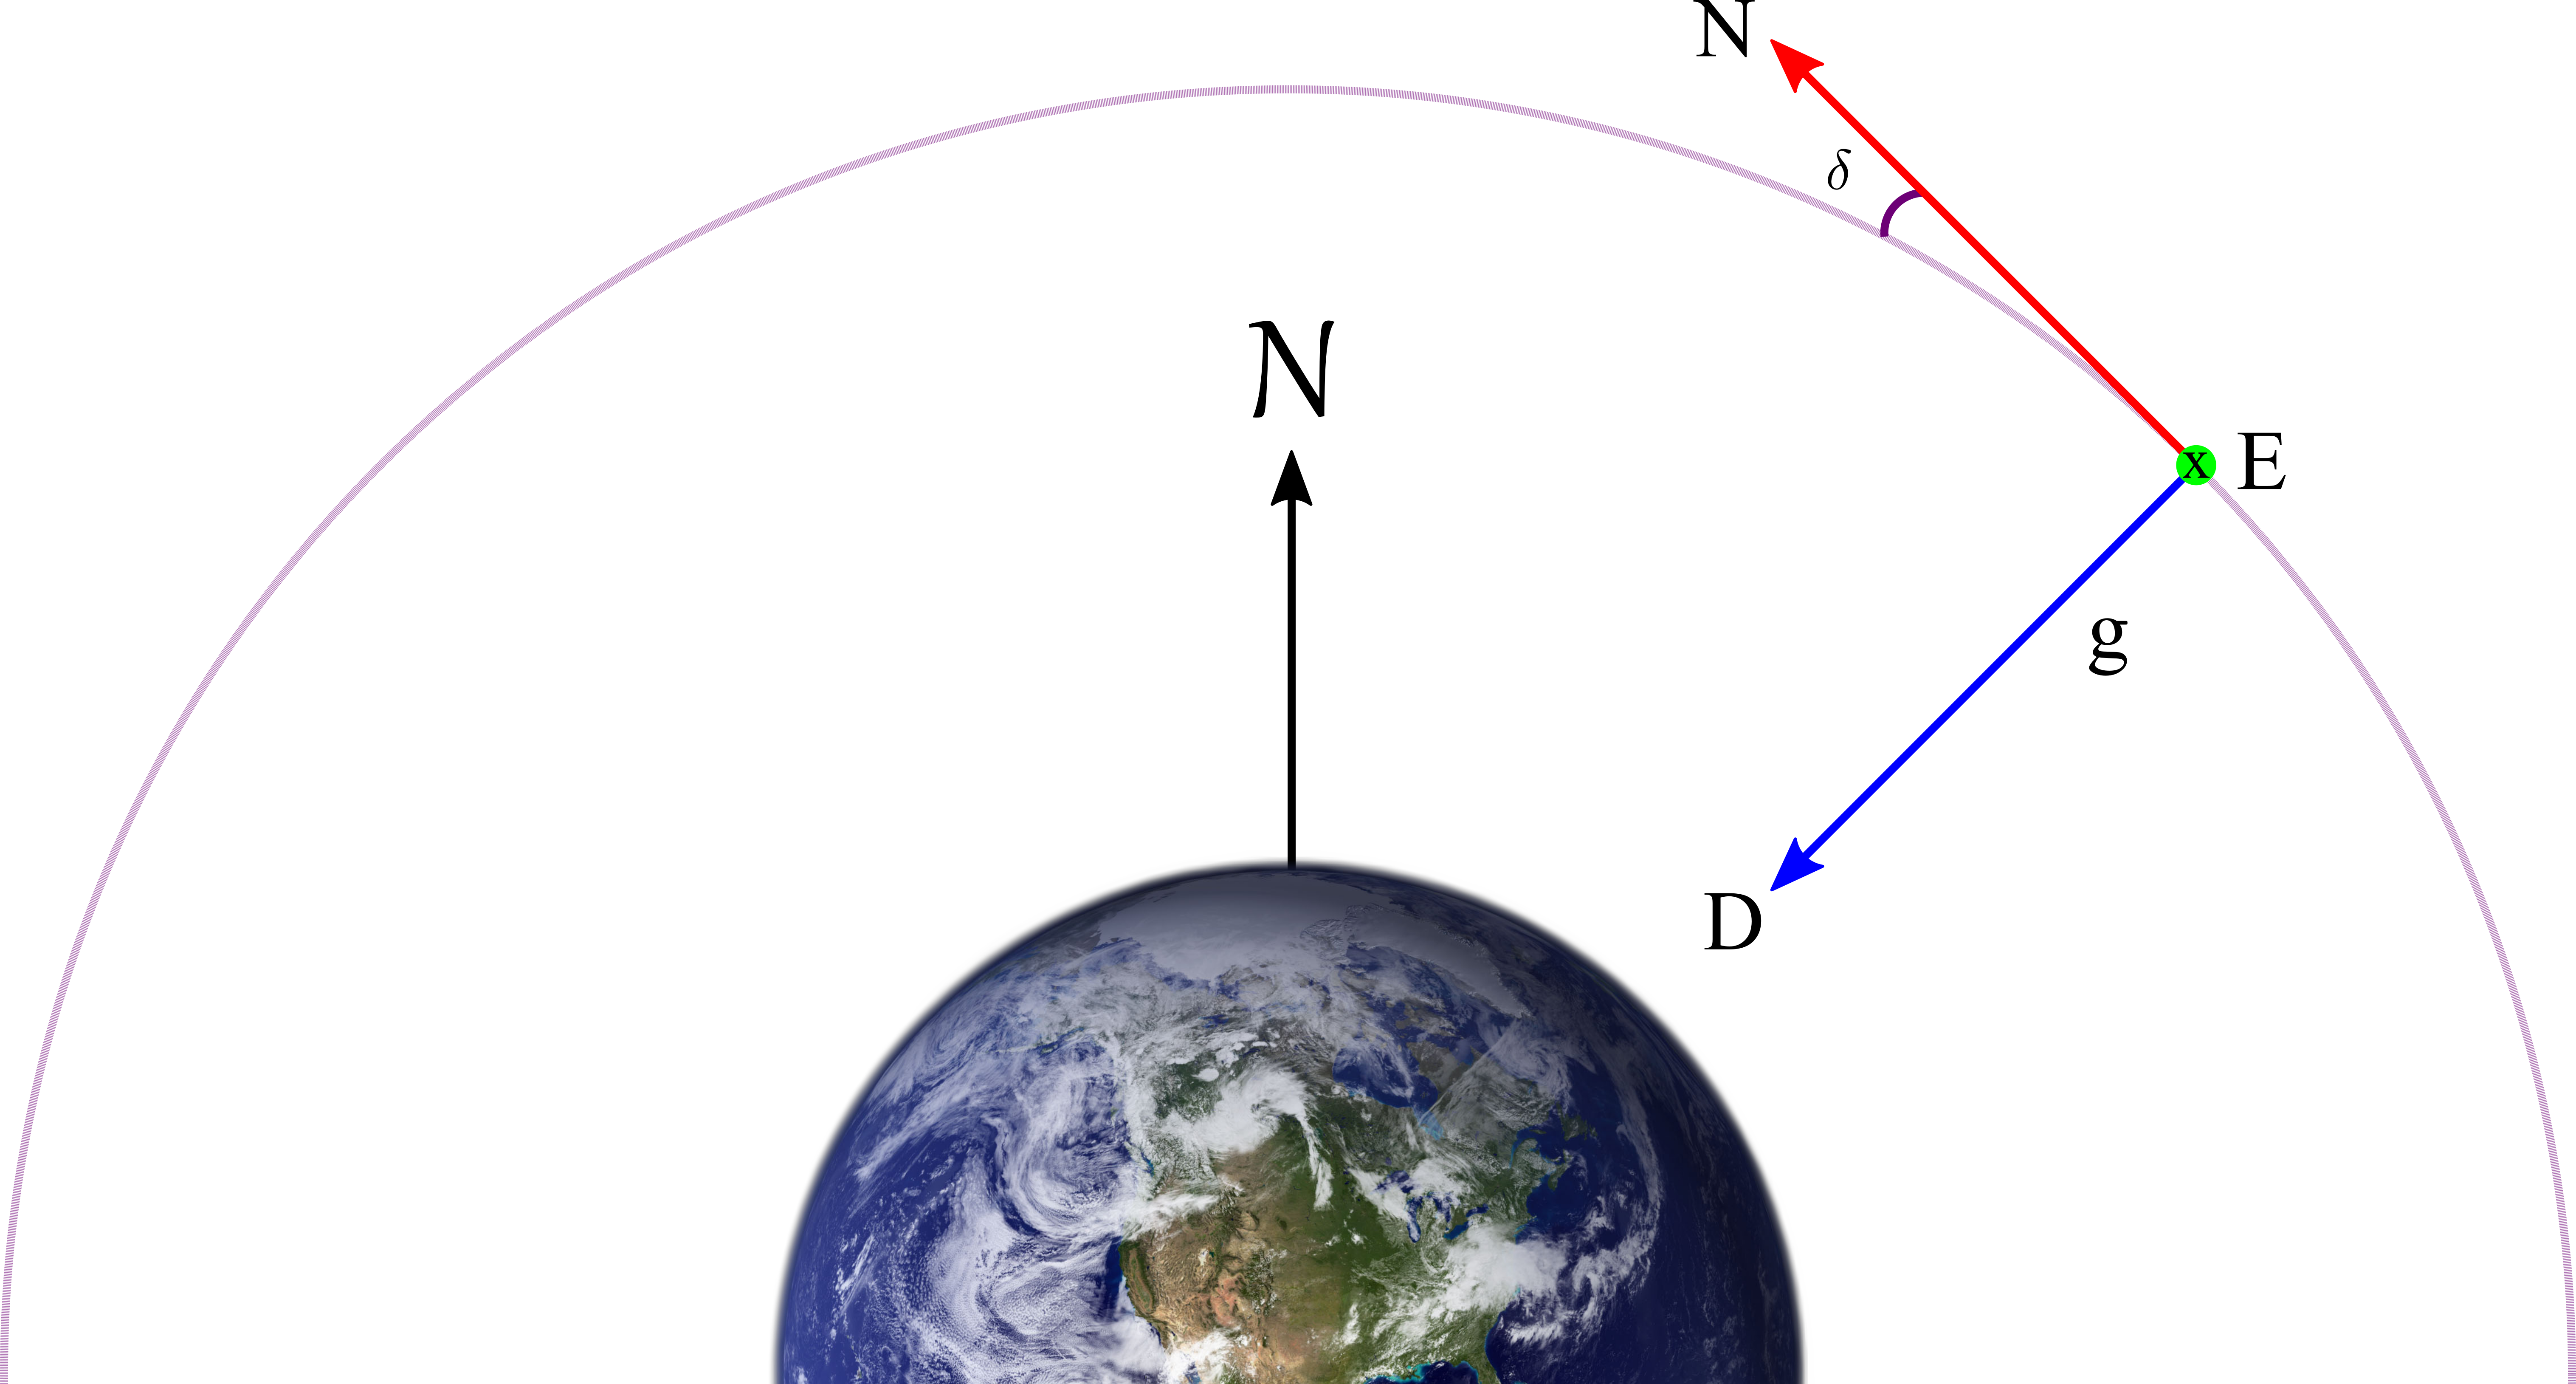
\includegraphics[width=8cm]{figs/fig_ned_frame.png}
    \caption{NED frame (N).}
    \label{fig_ned}
\end{figure}

NED (North-East-Down) frame is the local cartesian coordinate system that is that is established where the body is in space. The origin of the NED frame aligns with in the origin of body fixed frame. Axes x-axis, y-axis and z-axis are aligned towards North, East and down respectively where down referes to the vector pointing towards the centre of the Earth.

\section{Euler Angles and Rotation Matrix}
\label{sec_ypr}
Euler angles are used to parameterize rotation using three numbers: roll, pitch and yaw. Roll $\phi$, pitch $\theta$ and yaw $\psi$ represents the rotation about x-axis, y-axis and z-axis respectively. \medskip 

It is very important to mention the sequence of rotation when working on Euler angles and in this report we have used yaw-pitch-roll (3-2-1) sequence. This means that any arbitrary rotation of body frame from NED is expressed as the result of consecutive rotations about Z-axis, Y-axis and X-axis i.e. yaw, pitch and roll. Whenever Euler angles is mentioned from this point on, we mean 3-2-1 Euler angles unless otherwise stated. \medskip

Many practical problems requires the working with the rotation matrices. So we need to be able to convert the Euler angles to rotation matrix. Let us suppose rotation matrix $\bm{Q}(\psi,\theta,\phi)$ represents the rotation of body frame with respect to some inertial frame. The rotation matrix itself is composed of matrix multiplication of three rotation matrices that represents consecutive yaw, pitch and yaw. It can be written as:
\begin{equation}
\begin{split}
\bm{Q}(\psi,\theta,\phi) &= \bm{Q}_{\phi}\,\bm{Q}_{\theta}\,\bm{Q}_{\phi} \\
&=
\begin{bmatrix}
1 & 0 & 0 \\
0 & \cos{\phi} & \sin{\phi} \\
0 & -\sin{\phi} & \cos{\phi}
\end{bmatrix}
\begin{bmatrix}
\cos{\theta} & 0 & -\sin{\theta} \\
0 & 1 & 0 \\
\sin{\theta} & 0 & \cos{\theta}
\end{bmatrix}
\begin{bmatrix}
\cos{\psi} & \sin{\psi} & 0 \\
-\sin{\psi} & \cos{\psi} & 0 \\
0 & 0 & 1
\end{bmatrix} \\
&= \begin{bmatrix}
\text{c}\theta\,\text{c}\psi & \text{c}\theta\,\text{s}\psi & -\text{s}\theta \\
\text{s}\phi\,\text{s}\theta\,\text{c}\psi - \text{c}\phi\,\text{s}\psi & \text{s}\phi\,\text{s}\theta\,\text{s}\psi + \text{c}\phi\,\text{c}\psi & \text{s}\phi\,\text{c}\theta \\
\text{c}\phi\,\text{s}\theta\,\text{c}\psi + \text{s}\phi\,\text{s}\psi & \text{c}\phi\,\text{c}\theta\,\text{s}\psi -\text{s}\phi\,\text{c}\psi & \text{c}\phi\,\text{c}\theta
\end{bmatrix}
\end{split}
\end{equation}

\paragraph{Example} Let us suppose a body frame has orientation of $\psi = 45^{\circ}$, $\theta = 35^{\circ}$ and $\phi = 12^{\circ}$ (3-2-1 sequence) then the rotation matrix that can rotate the vector in inertial frame $\bm{v}^{I}\in \mathbb{R}^{3}$ to corresponding vector in body frame $\bm{v}^{B}\in \mathbb{R}^{3}$ by

\begin{equation}
\bm{v}^{B} = \bm{Q}(12^{\circ},35^{\circ},45^{\circ})\,\bm{v}^{I}
\end{equation}

\end{document}